\documentclass[a4paper,11.5pt]{article}
%\documentclass[a4paper,11pt]{scrartcl}

\usepackage{graphicx}
\usepackage[latin1]{inputenc}
\usepackage[italian]{babel}
\usepackage{fancyhdr}
\usepackage{amssymb}
\usepackage{makeidx}
\usepackage{eurosym}
\usepackage{alltt}

\usepackage{amsthm}

\theoremstyle{definition}
\newtheorem{defn}{Definizione}[section]



\title{Appunti di Progettazione Hardware 1}
\author{Matteo Gianello}
\date{\today}

\pdfinfo{%
  /Title    (Appunti di Progettazione Hardware 1)
  /Author   (Matteo Gianello)
  /Creator  (Matteo Gianello)
  /Producer ()
  /Subject  ()
  /Keywords (Basi Dati 2 Ferrandi IngInf Polimi)
}

\begin{document}
\pagestyle{empty}
\thispagestyle{empty}
\maketitle
\newpage

\thispagestyle{plain}
\tableofcontents
\newpage

\pagestyle{plain}
\label{capitolo1}
\section{Introduzione}
\subsection{Progettazione Hardware 1}
Nel corso di progettazione hardware 1 si tratter� la progettazione di sistemi complessi, non � solo a livello di VHDL, ma in realt� si tratteranno le metodologie di progettazione hardware e gli algoritmi per tale progettazione.\\
Si tratteranno diversi aspetti del flusso di progettazione ovvero:
\begin{itemize}
\item Sintesi dei sistemi digitali: progettazione e costruzione del sistema
\item Collaudo: fase tipica della progettazione hardware che non coincide con la verifica della corretta funzionalit� del sistema rispetto alle specifiche.
\item Verifica dei sistemi: questa � la vera fase di debug e di validazione rispetto alle specifiche.
\end{itemize}
I prerequisiti del corso sono la conoscienza degli argomenti trattati durante il corso di Reti Logiche. 
L'esame si compone di una prova scritta della durata di un'ora e un quarto, composta da 4/5 esercizi per un totale di 32 punti.
\subsection{Progettazione Hardware 2}
Nato da un corso tenuto da docenti di architetture, tenta di presentare lo sviluppo di hardware e software partendo da una specifica che non definisce la distribuzione dei compiti tra hardware e software.\\
Dove per software si parla di sistema dedicato. Mentre per hardware si intende una periferica (acceleratori hardware).
Gli argomenti trattati nel corso sono:
\begin{itemize}
\item Fase di specifica e modellazione di un sistema: modellazione di un sistema fisico di tipo digitale (che cos'� un modello di computazione e comunicazione?) prestanto particolare attenzione ai problemi di determinismo, parallelismo e concorrenza.
\item Progettazione e co-design: progettazione contemporanea di hardware e software (Problematiche di partizionamento, mapping delle risorse da usare).
\item Co-simulazione a livello di sistema (dipende dal tempo a disposizine del corso).
\end{itemize}
Preriquisiti di progettazione hardware 2 sono gli argomenti trattati in architetture avanzate dei calcolatori e reti logiche.
L'esame � composto da un test a risposta multipla che genera met� della valutazione finale mentre la seconda met� sar� assegnata previa realizzazione di un progetto che pu� essere di due tipi:
\begin{itemize}
\item Sviluppo di uno componente da integrare in un software per la progettazione assistita (CAD) da sviluppare in cpp.
\item Ricerca bibliografica su un argomento assegnato dal docente.
\end{itemize} 
\section{Introduzione PHW1}
Negli ultimi anni la complessit� dei progetti hardware � di molto incrementata, mentre i tempi per la loro realizzazione si sono ridotti drasticamente.
Per sopperire a queste mancanze la grandezza dei gruppi di lavoro � aumentata in maniera esponenziale, con progettisti con diverse capacit� che lavorano in parallelo a diversi livelli di astrazione.
La gestione delle complessit� e delle comunicazioni di progetto � arrivata ad un punto critico e gli strumenti di progettazione e di sintesi anche se molto evoluti sono inadeguati allo sviluppo di tali progetti costringendo il progettista ad usare fino a 50 strumenti differenti.
La sfida principale nella progettazione di un nuovo hardware si focalizzano principalmente sull'individuare il giusto compromesso tra time-to-market e costo/prestazioni.
La simulazione � ancora il principale mezzo per la verifica funzionale del progetto ma molto spesso � inadeguata rispetto alle dimensioni dello stesso.\\
Vi � un thrade of per quanto riguarda i modelli ad alto livello e quelli dettagliati; i modelli ad alto livello sono facili da mantenere ma omettono una grande quantit� di informazioni rendendo cos� le simulazioni molto veloci. I modelli pi� dettagliati richiedono un partizionamento maggiore aumentando i costi di comunicazione, inoltre, pur essendo pi� facili da maneggiare e ottimizzare richiedono tempi di simulazione molto lunghi.
Per questo i progettisti sono soliti dividere il problema in sottoproblemi pi� semplici e facili da controllare, dal sottoproblema individuano una soluzione tenedo conto delle condizioni di contorno e costruendo delle interfacce per lo scambio dei dati tra i componenti.\\
Una buona integrazione tra gli strumenti di progettazione e metodologie di progetto comporta comporta indirizzare la complessit� algoritmica mediante la suddivisione da parte dei progettisti del problema e l'indirizzamento degli strumenti automatici in base all'esperienza dei progettisti.\\


\label{capitolo2}
\section{Metodologie di progetto HW}
Nella progettazione hardware si segue un flusso di progettazione che sfrutta diversi livelli di astrazione. Questo flusso permette di partire da una specifica ad alto livello fino ad arrivare alla vera progettazione del sistema.
I progettisti non si occupano dello sviluppo del sistema completo ma si innestano a un certo livello per progettare un singolo componente/funzione.\\
Partiamo perci� dal contesto generale per spingerci poi a livello pi� piccolo.
Ma prima di definire quali sono i flussi di progetto devo definire quali sono gli elementi che compongono questo flusso.
\subsection{Dominio di rappresentazione dei circuiti}
Dal 1986/87 si � passati dalla descrizione di un sistema come una rete di componenti, alla descrizione di tale sistema attraverso un linguaggio di descrizione.
Domini di rappresentazione servono a identificare la complessit� della descrizione nei diversi domini.
%FIGURA DIAGRAMMA Y
Il diagramma  a Y ripartisce lo spazio di progetto in tre parti:
\begin{itemize}
\item Dominio fisico: moduli posizionamento piastre cabinet un buon modo per descrivere le fasi del progetto per individuare il punto ne quale ci si trova.
\item Dominio funzionale: � il dominio pi� vicino alle specifiche nel quale io specifico il comportamento del sistema. Si parte da una descrizione a livello di sistema che da una specifica ad altissimo livello descrive il comportamento del sistema (il tempo � trascurato); fino al livello di espressione logiche.
\item Dominio strutturale: Uno schema logico del sistema che specifica l'interconnesione dei vari componenti per formare il sistema completo. Si considerano soltanto gli aspetti di interconnesione nel sistema.
\end{itemize}
I cerchi concentrici servono per individuare i vari livelli di progettazione da quello pi� esterno che � quello pi� astratto a quello pi� interno che � quello  pi� specifico fisico.\\
Man mano che scendo nei livelli di astrazione il mio progetto diventa sempre pi� complesso ma comunque gestibili in quanto il sistema ad alto livello non � cambiato.\\
Il passaggio da una vista ad un'altra � chiamato sintesi; � il passaggio da il livello funzionale a livello strutturale a parte nel caso del passaggio dal dominio funzionale a quello fisico chiamata sintesi circuitale.
\subsubsection{Sintesi}
Cosa vuol dire fare sintesi? Vuol dire passare dalla descrizione del sistema ad un livello che � il pi� astratto possibile e via via dettagliarlo scendendo di livello. Partendo dal dominio funzionale a quello strutturale a quello fisico per ogni livello di astrazione.
Per la verifica (collaudo) si cerca di anticipare sempre pi� il momento della verifica in modo da individuare sempre prima la presenza di errori.
\begin{description}
\item[System Level]: Livello di descrizione del sistema in base alla sue funzionalit�, descrizione molto astratta simile a quello utilizzato nei linguaggi di programmazione.
\item[RT Level]: modello accurato vicino all'implementazione hardware con costrutti sequenziali per modellizzare costrutti pi� complessi come il \textit{while}. Manca ancora per� l'idea di tempo.
\item[Livello Logico]:livello di definizione nel quale vengono descritte le funzionalit� del sistema a livello di porte logiche e registri
\item[Transitor Level]:Applicazione a livello di transistor (solitamente CMOS); in questo caso possiamo avere diversi modelli in base alle applicazioni, functional equivalent checking o analisi timing accurata (tramite equazioni differenziali).
\item[Layout level]: Siamo al livello pi� basso dove i transistor sono visti come dei poligoni disposti sui diversi strati. Qui sono presenti le metallizzazioni e le diffusioni.
\end{description}
\subsection{Fasi di progetto}
Le fasi di progetto non sono isolate ma sono in parte sovrapposte o comunque esistono dei circoli tra le fasi.
Per quanto riguarda i costi le prime fasi tendono a essere meno costose in quanto le simulazioni sono veloci e semplici; gi� a livello RTL per� i costi aumentano in quanto si aggiungono molte complessit� come la temporizzazione.
Il flusso di progetto si pu� dividere in due macrofasi in quanto la seconda fase � gi� ben definita: front-end che comprende il "System level", il "Register transfert level" e il "Logic level"; e il back-end che comprende il Transistor, il Layout ed il Mask level.\\


\label{capitolo3}
\section{Analisi temporale}
Durante il corso di reti logiche abbiamo visto metodi di ottimizzazione che riguardano la minimizzazione dell'occupazione spaziale del circuito; nel caso in cui dovessimo ottimiziare il tempo di esecuzione per� le tecniche studiate non sono adatte.\\
Introduciamo alcune definizioni:
\begin{description}
\item[$A_k$:] tempo di arrivo (Arrival time)
\item[$R_k$:] tempo richiesto (Required time) � il tempo che si richiede per completare la computazione ed avere un risultato stabile all'uscita.
\item[$S_k$:] scarto (Slack) ovvero differenza tra  tempo richiesto e tempo di arrivo; se questa quantit� � negativa allora il progetto non soddisfa i vincoli temporali.
\end{description}
Introduciamo ora due modelli che rappresentano in diversa maniera il ritado temorale.
Il primo presenta un grafo con n nodi ai quali viene associato un certo ritardo e nel quale entrano un certo numero di ingressi. In questo caso il massimo tempo di uscita � dato dal massimo tempo di ingresso al nodo pi� il tempo di attraversamento del nodo $A_k=max(A_1,A_2,A_3)+D_k$.\\
Nel secondo modello, invece, il tempo di esecuzione � spostato sugli archi di ingresso; anche in questo caso da il tempo di uscita � dato dal massimo tra i tempi di ingressi $A_k=max(A_1+D_k,A_2+D_k,A_3+D_k)$.\\
\begin{figure}[hbt]
\centering
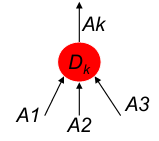
\includegraphics[width=5cm]{img/ritardo.png}
\caption{Esempio di ritardo di computazione}
\label{fig:ritardo}
\end{figure}
\subsection{Analisi statica}
Per calcolare il percorso critico di un circuito devo fare prima un preprocesso che calcola la massima distanza di ogni nodo dagli ingressi primari tramite l'algoritmo \textbf{LEVEL} che parte dai nodi di uscita e calcola in maniera ricorsiva che restituisce il distanza di ciascun nodo nel caso questo sia stato calcolato altrimenti richiama l'algoritmo per ogni nodo di ingresso. Dopodich� si calcola il tempo di arrivo (\textit{arrival time}) tramite l'algoritmo \textbf{ARRIVAL} che, sfruttando l'ordinamento topologico del primo algoritmo, calcola successivamente il tempo di arrivo al nodo di uscita partendo da quelli di ingresso.\\
\begin{verbatim}
// level of PI nodes initialized to 0, 
// the others are set to -1. 
// Invoke LEVEL from PO 
Algorithm LEVEL(k) { // levelize nodes
	if( k.level != -1) 
		return(k.level)
	else
		k.level = 1+max{LEVEL(k_i)|k_i fanin(k)}
	return(k.level) 
}
// Compute arrival times:
// Given arrival times on PI 
Algorithm ARRIVAL() {
	for L = 0 to MAXLEVEL
		for {k|k.level = L}
			A_k = MAX{A_ki} + D_k
}
\end{verbatim}
\subsection{Required Times}
Una volta calcolati i tempi di ingresso si procede ad analizzare il require time, ovvero i tempi ai quali � necessario avere i valori in uscita. I require time � una specifica del progetto. A questo punto vorrei sapere anche quali sono i require time all'interno della rete per individuare i punti critici del sistema. Per fare ci� si procede calcolando il require time ad un nodo come require time all'uscita del nodo successivo meno tempo di attraversamento del nodo successivo e tra tutte le uscite prendo il minimo.
Il seguente sistema specifica in modo matematico le specifiche del sistema tramite lo slack ovvero la differenze tra require time ed arrival time.
Nel caso questo sia negativo ho trovato un percorso critico del sistema.
$$
\begin{array}{rcl}
S_k & = & R_k-A_k\\
R{m,k}&=&R_k-A_k\\
A_k&=&max\{A_{ki}\}+D_k\\
S_{m,k}&=&R_{m,k}-A_m\\
S_{m,k}&=&S_k+max\{A_ki\}-A_m\\
S_m&=&min\{S_{m,kr}\}\\
\end{array}
\begin{array}{rcl}
k_i,m &\in& fanin(k)\\
k_r &\in& fanout(m) 
\end{array}
$$
Un percorso critico � un percorso $P=\{i_1,i_2,\dots,i_p \mbox{ dove } S_{i_k,i_{k+1}}<0$.
Il problema di ottimizzazione della static time analysis si riduce a trovare il percoso con slack negativo pi� grande in valore assoluto, ovvero minimizzare $max\{-S_i,0\}$.
Veniamo ora al perch� vi � la necessit� di effettuare un'analisi temporale del circuito. Lo scopo principale � quello di stimare quando l'uscita del circuito diventa stabile e perci� verificare la correttezza del mio dispositivo.
Inoltre l'analisi temporale permette di individuare dove � pi� efficace effettuare delle ottimizzazioni e vedere dove il sistema non rispetta i vincoli temporali.\\
Esistono diversi metodi per effettuare time analysis il metodo pi� grezzo per  effettuare l'analisi temporale � effettuare una simulazione con tutti i vettori di input; ma questa tecnica risulta essere molto dispendiosa. Perci� il metodo che utilizzeremo sar� l'analisi temporale a livello di gate.\\
Prima di procedere per� dobbiamo effettuare alcune ipostesi; la prima � quella di avere una caratterizzazione predefinita dei ritardi delle porte logiche e la seconda quello di effettuare la simulazione a livello logico.
I problemi principali di questo tipo di analisi sono l'individuazione dei \emph{false path} ovvero di quei percorsi che non vengono attivati qualsiasi siano i vettori di input, in modo da eliminarli in quanto non vengono mai attivati e concentrarsi su quelli attivi. Altrimenti avremmo una stima per eccesso del ritardo.
\subsection{Analisi statica}
\subsubsection{Analisi dei false path}
L'analisi dei false path serve ad individuare quei percorsi che non vengono attivati durante l'esecuzione dei programmi in modo da non doverli conteggiare nel calcolo dei ritardi nei percorsi critici. Questa analisi � complessa ma permette, almeno, di non sottostimare il tempo di ritardo e di sovrastimarli leggermente.\\
Per effettuare l'analisi dei false path devo andare ad individuare le condizioni che mi permettono di tenere attivo tutto il percorso; qlcune di queste condizioni sono molto semplici da individuare se teniamo conto che il nostro circuito � creato da sole porte AND e OR.
Introduciamo il concetto di valore controllante per una porta logica; per valore controllante si intende un valore che applicato ad una porta logica permette di conoscere il risultato in uscita senza conoscere il valore dell'altro ingresso. Nel caso di una porta AND il valore controllante � 0 mentre per una porta OR � 1 come mostrato in tabella \ref{tab:valoricont}
\begin{table}[t]
\centering
\begin{tabular}{|c|c|c|}
\hline
Porta&Valore controllante&Valore non controllante\\
\hline
AND&0&1\\
\hline
OR&0&1\\
\hline
\end{tabular}
\caption{Tabella dei valori controllanti e non controllanti per le porte AND e OR.}
\label{tab:valoricont}
\end{table}
\subsubsection{Statically-sensitizable}
Ora per� sorge la domanda se il false path individuato non influisce realmente sul ritado di computazione. Per individuare ci� si usa la \emph{statically-sensitization analysis}.\\
Un percorso si definisce \emph{statically-sensitizable} se esiste un vettore di input che imposta a tutte le porte, che ricevono in ingresso un input, un valore non controllante indipendentemente dal ritardo delle porte.
Il percorso pi� lungo individuato �  il \emph{il percorso pi� lungo attivabile}.\\
Questa affermazione � vera finche non introduciamo i ritardi delle porte.
Infatti � possibile che una porta abbia un valore controllante ad un certo istante di tempo e un valore non controllante in un altro istante di tempo come nell'esempio di fig.\ref{fig:timesim}
\begin{figure}[ht]
\centering
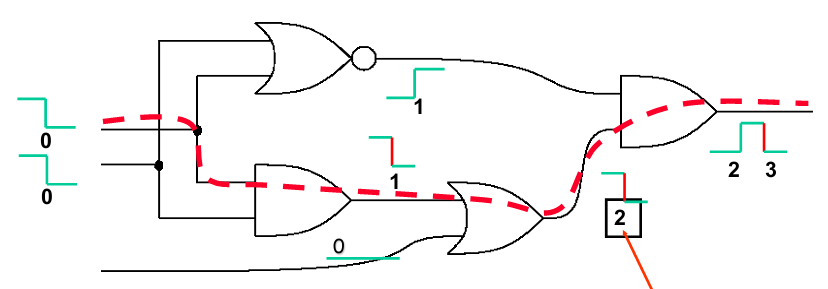
\includegraphics[width=16cm]{img/timesim.png}
\caption{Esempio di valore non controllante ad un certo istante di tempo}
\label{fig:timesim}
\end{figure}
\subsubsection{Timing Simulation}
Nella timing simulation si imposta un vettore di ingresso e si simula il circuito tenendo conto dei ritardi delle porte come in  figura \ref{fig:timing1}
\begin{figure}[thb]
\centering
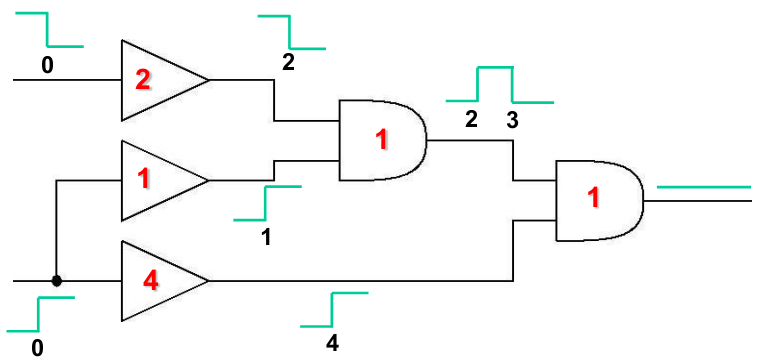
\includegraphics[width=11cm]{img/timing1.png}
\caption{Esempio di timing simulation}
\label{fig:timing1}
\end{figure}
Questo meccanismo � un po impreciso infatti il ritardo delle porte � una quantit� variabile $[0,d]$ dove d � il ritardo massimo.
Come si vede dalla figura \ref{fig:timing2} diminuire il ritardo delle porte pu� portare ad aumentare il ritardo complessivo del percorso. Questo aspetto viola la regola dello speedup monotono. Tale regola afferma che dato un circuito C e un circuito C\' ottenuto da C riducendo il ritardo di alcune porte allora il ritardo complessivo deve essere minore di quello di C.
\begin{figure}[thb]
\centering
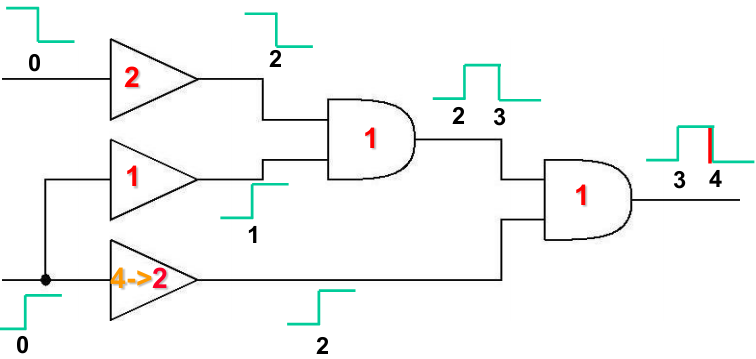
\includegraphics[width=11cm]{img/timing2.png}
\caption{Esempio di timing simulation con riduzione dei ritardi}
\label{fig:timing2}
\end{figure}
\subsubsection{Simulazione X-Valued}
La simulazione X-Valued assomiglia molto alla simulazione "timing" in questo caso per� si trascurano i valori antecedenti all'istante di inizio simulazione; tale concetto � espresso da una notazione particolare mostrata in figura \ref{fig:xvalue}
\begin{figure}[thb]
\centering
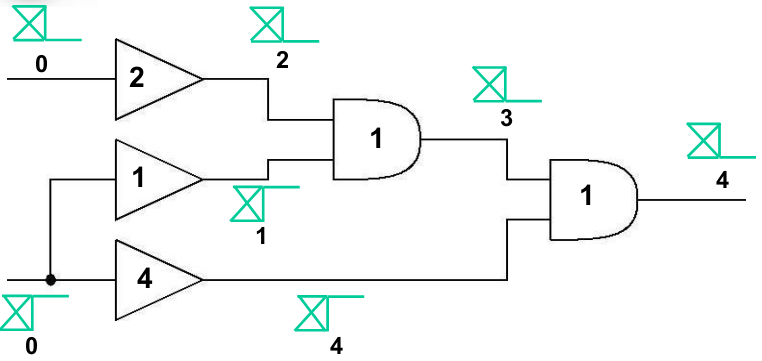
\includegraphics[width=11cm]{img/xvalue.png}
\caption{Esempio di X-Value simulation}
\label{fig:xvalue}
\end{figure}
In questo caso sappiamo che dall'istante successivo alla "X" il valore � stabile.
Questo tipo di simulazione � la pi� accurata per circuiti logici con porte semplici.\\
Per conoscere il vero valore del ritardo massimo devo per� provare tutti i diversi vettori di ingresso del circuito.
\subsubsection{Algoritmi di analisi dei percorsi critici}
Verificare la criticit� di ogni percorso di un circuito logico risulta essere troppo costoso; per fare un esempio analizziamo quale sarebbe il procedimento (ricerca per bisezione).
\begin{verbatim}
Start: set L = L_top /* = topological longest path delay */
L_old= 0
2. Binary search: 
If (Delay(L))
	!L = |L-L_old|/2, L_old = L, L = L-!L
Else,  
	!L = |L-L_old|/2, L_old = L, L = L +!L
If (L > L_top or !L < threshold), L = L_old
\end{verbatim}
La funzione \emph{Delay(L)} � uguale a 1 se esiste un vettore di ingresso tale che fa si che l'uscita sia stabile solo dall'istante t tale che $L\leq t$. Questo problema pu� essere risolto con due metodi:
\begin{itemize}
\item SAT problem
\item timed-ATPG
\end{itemize}
\subsection{SAT based False path analysis}
L'analisi dei percorsi critici attraverso il metodo SAT permette di determinare se esistono dei vettori di ingresso per cui l'uscita � stabile al tempo t=T e se questo insieme di vettori comprende l'insieme dei vettori positivi che posso applicare al circuito.
Per fare ci� basta prendere la funzione caratteristica di S(insieme dei vettori che soddisfa la condizione) e di S(T) (insieme dei vettori che non soddisfa la condizione) allora se $F\wedge!F(T)=\emptyset$ allora non esiste nessun vettore che rende non stabile l'uscita dopo T (F e F(T) funzioni caratteristiche rispettivamente di S e S(T)).
L'idea � quella di verificare se esiste un certo istante T tale per cui $S(T)=S$ dove S � l'insieme di tutti i vettori di ingresso.
\paragraph{Esempio}
Prendiamo in considerazione il circuito di figura \ref{fig:sat1}
Vogliamo verificare se esiste un qualche vettore di ingresso per cui l'uscita non � stabile ad un tempo $t>2$.
\begin{figure}[hbt]
\centering
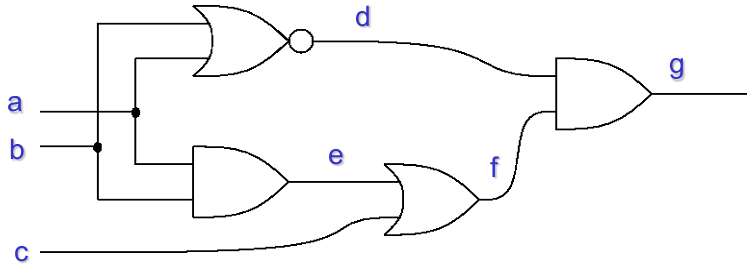
\includegraphics[width=12cm]{img/sat1.png}
\caption{Esempio di analisi con il metodo SAT}
\label{fig:sat1}
\end{figure}
Dividiamo il problema in due sottoproblemi, il primo nel caso l'uscita sia uguale a 1 e il secondo nel caso l'uscita sia uguale a 0
Verifichiamo ora che l'uscita � uguale a 1 al tempo t=2.
Per fare ci� calcoliamo la funzione caratteristica $g(1,t=2)$ che calcola i vettori di ingresso che rendono stabile l'uscita all'istante t=2.
$$
\begin{array}{rcl}
g(1,t=2)&=&d(1,t=1)\cap f(1,t=1)\\
&=&(a(0,t=0)\cap b(0,t=0))\cap (c(1,t=0)\cup e(1,t=0))\\
&=&!a!b(c\cup \emptyset)=!a!bc=S_1(t=2)
\end{array}
$$
La funzione caratteristica � una funzione utilizzata per rappresentare in modo insiemistico le funzioni logiche nel quale l'OR � l'unione l'AND l'intersezione.\\
Calcoliamo ora l'onset del circuito ovvero quali valori rendono stabile l'uscita in qualsiasi istante di tempo. la funzione caratteristica dell'onset � indicata da $g(1,t=\infty)$. In questo esempio �:
$$
g(1,t=\infty)=!a!bc=g(1,t=2)=S_1
$$
Il fatto che i due insiemi siano uguali fa si che per l'uscita uguale a 1 non esistono vettori di ingresso che rendono l'uscita stabile a un tempo $t>2$.\\
Ora dobbiamo applicare i ragionamenti precedenti anche per l'uscita stabile al valore 0. Quindi calcoliamo la funzione caratteristica all'istante 2 e all'istante infinito.
$$
\begin{array}{rcl}
g(0,t=2)&=&d(0,t=1)\cup f(0,t=1)\\
&=&(a(1,t=0)\cup b(1,t=0))\cup (c(0,t=0)\cap e(0,t=0))\\
&=&a+b+(!c\cap \emptyset)=a+b=S_0(t=2)
\end{array}
$$
Mentre l'offset del circuito �:
$$g(0,t=\infty)=offset=a+b+!c=S_0$$
$$g(0,t=\infty)/g(0,t=2)=(a+b+!c)!(a+b)=!a!b!c$$
Questo significa che per il vettore di ingresso [0,0,0] l'uscita non � stabile al tempo 2.
\subsection{Ottimizzazione Combinatoria}
I fattori che determinano il ritardo in un circuito si possono suddividere in 3 categorie a loro volta suddivisibili in sottocategorie:
\begin{itemize}
\item fattori che riguardano la tecnologia del circuito:
	\begin{itemize}
		\item Tipo di tecnologia utilizzata per la costruzione del circuito
		\item Tipo di gate 
		\item La dimensione dei gate pi� grandi danno prestazioni migliori
	\end{itemize}
	\item fattori che riguardano la struttura logica del circuito:
	\begin{itemize}
		\item La lunghezza dei percorsi di computazione.
		\item I false path.
		\item Meccanismi di buffering.
	\end{itemize}
	\item fattori parassitari:
	\begin{itemize}
		\item Layout del circuito.
		\item Capacit� parassite.
	\end{itemize} 
\end{itemize}
Lo scopo dell'ottimizzazione combinatoria � quello di partire dalla descrizione iniziale del circuito con i suoi vincoli, dalla lista delle specifiche e da una serie di librerie e funzioni primitive per arrivare a un'implementazione del circuito con queste librerie che rispetti i vincoli di prestazioni e che sia minimizzata in termini di area.\\
Esistono diversi approcci per ottenere i risultati richiesti; alcuni approcci sono locali ovvero ottimizzano solo una parte del circuito mentre altri approcci sono globali. I principali approcci locali sono:
\begin{itemize}
\item il trasporto in avanti (THR)
\item la somma condizzionale (GST)
\item il trasporto sul bypass (GBX e KMS)
\end{itemize}
I primi due puntano sull'ottimizzazione dei livelli e quindi pi� improntati ad una ottimizzazione dell'area mentre il terzo � improntato sull'analisi dei false path.
\subsubsection{Tree-Height Reduction - THR}
La prima tecnica che analiziamo ha come principio quello di indivuduare i punti del circuito che violano i vincoli e ridurre questa parte.\\
Dati gli arrival time all'ingresso e i required time alle uscite individuo la zona critica che non rispetta i tempi; nel caso di fig. \ref{fig:thr} in cui la parte critica concorre al calcolo dell'uscita "m" trovo una sottoparte non critica che pu� essere duplicata e collaso il percorso che viola i vincoli  risintetizzandolo. La risintetizzazione avviene solo su una parte del circuito altrimenti dovrei riprogettare tutto con conseguenti costi di riprogettazione, aumento di area ecc.
\begin{figure}[t]
\centering
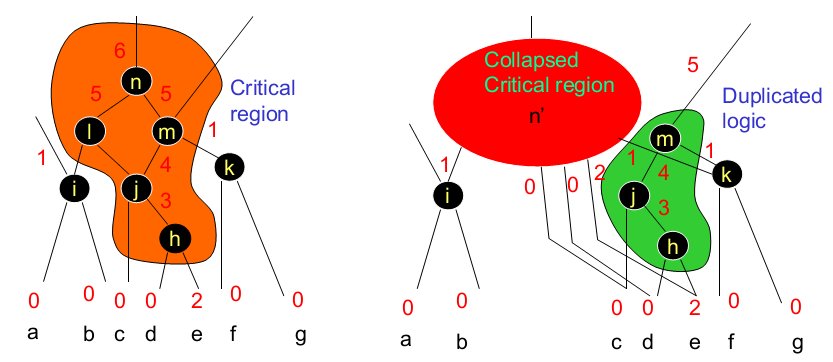
\includegraphics[width=16cm]{img/thr.png}
\caption{Esempio di THR}
\label{fig:thr}
\end{figure}
\subsubsection{GBX e KMS}
L'idea del GBX � quella di bypassare il percorso critico inserendo a livello dell'eventuale porta di attivazione del percorso critico un uscita collegata ad un multiplexer e comandata dal valore che attiverebbe il percorso critico rendendo cos� il circuito pi� veloce.\\
Il GBX comporta un piccolo aumento nell'area del circuito ed inoltre introduce un punto di non testabilit� sul valore controllante del multiplexer.\\
Si � cos� introdotto il meccanismo KMS che rimuove il percorso critico senza incrementare il ritardo. Per fare ci� si duplica il percorso critico fino all'ultimo nodo che contiene un \emph{fanout}; si inserisce inoltre un ingresso controllante sul primo nodo del percorso critico. Si ottiene cos� che le funzioni fino all'ultimo nodo con fanout non sono cambiate aggiungendo solo una piccola area al circuito.
\subsubsection{Generalized Select Transform}
Dato il percorso critico con due linee di ingresso delle quali una sola genera il percorso critico, in quanto il segnale arriva con un ritardo maggiore rispetto all'altro ingresso, allora si duplica tale percorso e si impongono all'ingresso dei due percorsi in un caso il valore 0 e nell'altro il valore 1 sulla linea che genera il percorso critico; si inserisce alla fine del percorso un multiplexer controllato dal valore della linea  duplicata. Questo meccanismo permette di anticipare il calcolo del percorso critico (vedi fig. \ref{fig:gst}).
\begin{figure}[t]
\centering
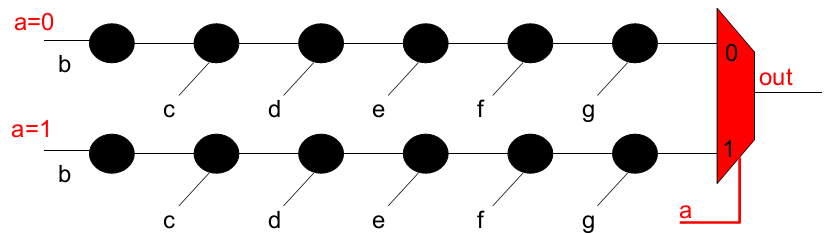
\includegraphics[width=16cm]{img/gst.png}
\caption{Esmpio di GST}
\label{fig:gst}
\end{figure}
\subsection{Ottimizzazione sequenziale}
L'ottimizzazione sequenziale tiene conto del tempo del circuito ed implica l'"introduzione" nel circuito di componenti atti a memorizzare lo stato passato del circuito.\\ Questo tipo di sintesi pu� essere applicata a diversi livelli di astrazione allontanandoci sempre pi� dal livello di sistema e avvicinandoci a quello fisico.\\ Questo implica un ottimizzazione migliore ma anche una maggior difficolt� di verifica.\\
Le due tecniche principali di ottimizzazione sono:
\begin{itemize}
\item \textbf{Clock Skew Scheduling} si tratta di una tecnica che mira a bilanciare il ritardi delle porte attraverso dei registri individuali.
\item \textbf{Retiming} tecnica che prevede di spostare i registri all'interno del circuito attuando inoltre delle ottimizzazioni combinatorie.
\end{itemize}
\subsubsection{Clock Skew Schedulig}
Il clock skew scheduling si basa sul presupposto che la parte combinatoria tra due registri deve terminare la sua esecuzione entro il tempo di clock per permettere il campionamento del segnale di uscita. Pi� alcune costanti.
\begin{figure}[hbt]
\centering
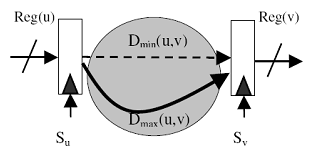
\includegraphics[width=16cm]{img/css.png}
\caption{Porta con meccanismo di clock skew scheduling}
\label{fig:css}
\end{figure}
Un circuito sequenziale sincrono pu� funzionare correttamente solo se vengono rispettati alcuni vincoli:
$$S_u+D_{max}(u.v)+ SETUP_v\leq S_v+T$$
$$S_u+D_{min}(u.v)\geq S_v+HOLD_v$$
Il primo vincolo � detto di \emph{zero-clocking} ed afferma che il segnale deve raggiunge il registro $v$ prima del segnale di clock successivo; il tempo per raggiungere il registro successivo � dato dal tempo di setup del registro di arrimo pi� il ritardo massimo della parte combinatoria.\\
Il secondo vincolo, invece, chiamato di \emph{double-clocking} specifica che il segnale in ingresso e in uscita � sicuro fino all'istante di clock overo che il segnale precedente duri al massimo fino al tempo di clock.\\
In un circuito sincrono con un clock \emph{zero-skew} $S_u$ e $S_v$ sono uguali  e questo implica che il minimo periodo di clock T � uguale al massimo valore di $D_{max}(u,v)+SETUP_v$ presente nel circuito.
Se il valore $S_u-S_v\leq 0$ il periodo di clock pu� essere minore del massimo ritardo del circuito.\\
Lo scopo dell'ottimizzazione � quello di determinare il valore appropriato di $S_u$ e $S_v$ per tutte le coppie di registri per ottenere il minimo periodo di clock.\\
I vantaggi di questa tecnica sono una meccanismo di post-sintesi per ridurre il periodo di clock praticamente gratuita e si mantiene il design del circuito.
I problemi principali invece sono che i vincoli devono essere rispettati, � impossibile mescolare questa tecnica con quelle di ottimizzazione combinatoria ed infine si tende ad avere una replicazione degli alberi di clock.
\subsubsection{Retiming}
\begin{figure}[thb]
\centering
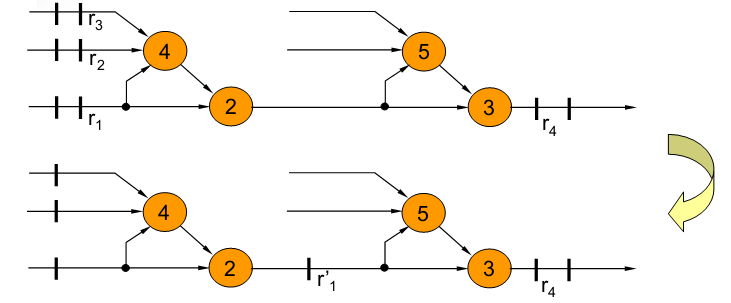
\includegraphics[width=16cm]{img/retiming.png}
\caption{Esempio di retiming}
\label{fig:retiming}
\end{figure}
Il retiming � una tecnica che consiste nello spostare prima o dopo il nodo alcuni buffer gia presenti nel circuito magari accorpando alcuni flip-flop. Questa tecnica risulta essere pi� semplice da attuare in quanto bisogna tenere in considerazione solo il vincolo di setup del buffer. Inoltre permette un'integrazione con altri metodi di integrazione sia sequenziale sia combinatoria per ottenere un ottimo globale. I punti a sfavore di questa tecnica sono il fatto che rendono pi� difficile la verifica e comportano un calcolo approssimativo del ritardo del circuito.\\
Il retiming pu� avere due obiettivi, il primo quello di minimizzare l'area accorpando i filip-flop e il secondo � quello di ridurre il tempo di clock; questi due obiettivi possono essere ottimizzati insieme e a quel punto si parla di \emph{Retiming con ottimizzazione combinatoria}.
Vediamo ora un algoritmo per il calcolo del retiming; rappresentiamo il circuito come un grafo $G(V,E,d,w)$ dove:
\begin{itemize}
\item $V\rightarrow$ � l'insieme delle porte
\item $E\rightarrow$ � l'insieme delle interconnessioni 
\item $d(v) =$ ritardo dei gate
\item $w(e) = $ numero di registri sull'interconnessione
\end{itemize}
Vediamo l'esepio in fig. \ref{fig:retalgo}
\begin{figure}[t]
\centering
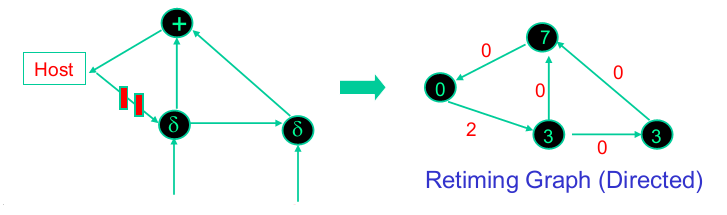
\includegraphics[width=16cm]{img/retalgo.png}
\caption{Esempio di creazione di un grafo per retiming}
\label{fig:retalgo}
\end{figure}
Dove $\delta$ ha un ritardo di tre e $+$ ha un ritardo di 7 unit� di tempo.Definiamo ora che cosa � un \emph{Percorso}, esso � un insieme di nodi ordinati del grafo con un nodo iniziale e uno finale.
Il \emph{ritardo} di un percorso � la somma dei ritadi di tutti i nodi estremi inclusi. Il \emph{peso} di un percorso � la somma dei pesi degli archi ovvero la somma dei flip-flop presenti sul percorso.\\
Dato il percorso:
$$v_0\rightarrow^{e_0}v_1\rightarrow^{e_1}\dots v_{k-1}\rightarrow^{e_{k-1}}v_k$$
Il suo ritardo �:
$$d(p)=\sum_{i=0}^kd(v_i)$$
Ed il suo peso �:
$$w(p)=\sum_{i=0}^{k-1}w(e_i)$$
A questo punto possiamo definire il periodo di clock del circuito come:
$$c= \max_{p:w(p)=0}\{d(p)\}$$
Significa che il massimo dei ritardi di tutti i percorsi con peso 0 definisce il ritardo massimo del circuito e quindi del periodo di clock.\\
Definiamo ora un operazioni di retimind uguale a $-1$ se sposto dei registri dagli ingressi alle uscite, un retiming uguale a $+1$ se sposto i registri dalle uscite agli ingressi.
Dati due nodi e l'arco ad esso associati definiamo il peso dell'arco dopo l'operazione di retiming come (fig. \ref{fig:retarc}):
$$w_r(e)= w(e) + r(v) - r(u)$$
dove $r(v)$ e $r(u)$ sono rispettivamente le operazioni di retiming sui nodi di uscita e quello di ingresso all'arco in esame.
\begin{figure}[t]
\centering
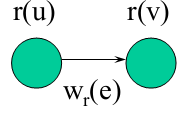
\includegraphics[width=7cm]{img/retarc.png}
\caption{Funzione di retiming}
\label{fig:retarc}
\end{figure}
Definiamo ora il problema di minimizzazione del ciclo di clock tramite retiming.
La funzione obiettivo � la minimizzazione del ritado massimo
$$\hbox{minimize}\; c = \max_{P:w_r(p) = 0}\{d(p)\}$$
Definiamo ora due matrici, la matrice dei pesi e la matrice dei ritardi
$$W(u,v) = \min_p{w(p):u\rightarrow^p v}$$
$$D(u,v) = \max_p{d(p):u\rightarrow^p v,w(p) = w(u,v)}$$
Nel caso in esempio abbiamo a che le due matrici sono cos� composte:
$$
W=
\begin{array}{cccc}
0&2&2&2\\
0&0&0&0\\
0&2&0&0\\
0&2&2&0\\
\end{array}
$$
$$D=
\begin{array}{cccc}
0&3&6&13\\
13&3&6&13\\
10&13&3&10\\
7&10&13&7\\
\end{array}
$$
La matrice \emph{W} mi identifica i percorsi critici mentre mentre la matrice \emph{D}, in corrispondenza dei percorsi nulli della matrice \emph{W} mi identifica il periodo di clock; mi basta prendere il massimo tra tutti i numeri che hanno come peso il valore 0.\\
Tutto questo mi aiuta ad ottimizzare il circuito tramite retiming; supponiamo di volere un determinato periodo di clock $T$ a questo punto dobbiamo applicare il retiming su quei percorsi che hanno un valore maggiore di $T$.
Per minimizzare il numero dei registri invece mi basta minimizzare la somma dei pesi degli archi.

\label{capitolo4}
\section{Tecnology Mapping}
Il tecnology mapping � una fase di ottimizzazione che si colloca sotto l'ottimizzazione tecnology indipendent. Questa operazione consiste nell'assegnare alle diverse funzioni logiche del circuito una serie di porte in base a delle librerie che contengono una serie di porte. Queste librerie vengono chiamate \emph{cell library}.
Esistono due approcci per effettuare il tecnology mapping il primo � abbastanza euristico basato su regole di sostituzione di tipo tecnology indipendent molto efficente per piccoli circuiti ma richiede un tempo eccessivo di computazione.\\
Il secondo approccio invece si basa su algoritmi; si divide in diversi passi primo dei quali � trasformare la rete attraverso una serie di funzioni base. Il grafo cos� formato viene detto \emph{subject graph} tipicamente formato solo da porte NAND a due ingressi e da inverter. Il secondo passo dell'algoritmo � rappresentare anche le funzioni di libreria mediante l'utilizzo di porte NAND e inverter, questo genera il cosidetto \emph{pattern graphs}
\begin{figure}[hb]
\centering
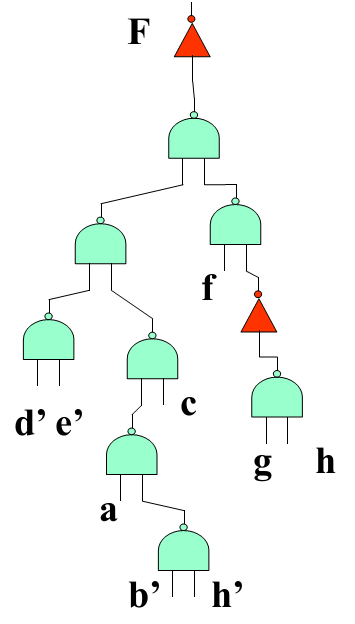
\includegraphics[height=9cm]{img/subject.png}
\caption{Esempio di subject graph}
\label{fig:subject}
\end{figure}
\subsection{algoritmo}
Terminata la fase di preparazione si passa alla fase in pi� propriamente algoritmica. Lo scopo � quello di effettuare la miglior \emph{copertura} del grafo, ovvero, fare in modo che ogni nodo del subject graph sia contentuto in uno o pi� pattern graph. inoltre ogni input di un pattern graph deve essere l'output di qualche altro grafo.\\
I diversi algoritmi devono trovare la copertura di costo minimo migliore per il subject graph sottoposto all'analisi.
\begin{figure}[thb]
\centering
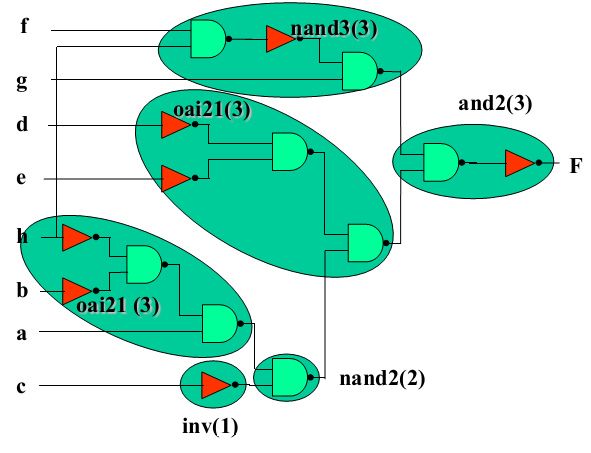
\includegraphics[width=10cm]{img/copertura.png}
\caption{Esempio di copertura con porte AND OR-AND a 2+1 ingressi e NAND a 3 ingressi}
\label{fig:copertura}
\end{figure}
\subsection{Copertura DAG}
Il tecnology mapping utilizzando il metodo DAG richiiede come ingresso la rete ottimizzata e descritta in modo indipendente dalla tecnologia e la libreria di porte da utilizzare. Esso restituisce la netlist di porte che minimizza il costo totale.\\
Il meccanismo � quello di verificare tutte le possibili combinazioni \{$m_k$\} per ogni nodo e impostando ($m_i=1$) tutte le variabili per il quale il pattern graph � scelto. Dopodiche si scrivono una serie di clausule per ogni nodo del subject graph indicando quali match sono stati effettuati. Ripetendo tale operazione per tutti i nodi e moltiplicando le varie clausule si ottiene la soluzione cercata
\begin{table}[hbt]
\centering
\begin{tabular}{c|c|c|c|c|}
&$m_1$&$m_2$&\dots&$m_k$\\
\hline
$n_1$&&&&\\
\hline
$n_2$&&&&\\
\hline
$\vdots$&&&&\\
\hline
$n_l$&&&&\\
\hline
\end{tabular}
\caption{Esempio di tabella di copertura}
\label{tab:t_copertura}
\end{table}
\subsection{Optimal tree covering}
Nel caso particolare in cui la nostra rete logica sia ad albero, ovvero non vi � la presenza di fanout esiste un algoritmo pi� efficente per trovare la copertura migliore.\\
Il principo � quello di coprire gli alberi in modo ottimale usando la programmazione dinamica. L'assunzione che si fa � che per ogni figlio dell'albero si conosce in modo ricorsivo il costo migliore per la copertura e si assume che gli ingressi abbiano costo 0. A questo punto il costo totale � dato dalla somma di tutti i costi.
\begin{verbatim}
Algorithm OPTIMAL_AREA_COVER(node) {
	foreach input of node {
		OPTIMAL_AREA_COVER(input);// satisfies recurs. assumption
	}
	// Using these, find the best cover at node 
	node->area = INFINITY;
	node->match = 0;
	foreach match at node {
		area = match->area;
		foreach pin of match {
			area = area + pin->area;
		}
		if (area < node->area) {
			node->owarea = area;
			node->match = match;
		}
	}
}
\end{verbatim}


\label{capitolo5}
\section{Sintesi ad alto livello}
I primi processi di automazione del desidn di cicruiti digitali tendevano a dare troppa enfasi agli aspetti incrementali degli algoritmi facendo assunzioni su componenti e ritardi non realistici generando circuiti di basso livello di scarsa qualit�\\
La sintesi architeturale di alto livello permette un innalzamento del livello di astrazione delle specifiche portando cos� a specifiche pi� snelle e pi� facilmente modificabili. Inoltre permette di ridurre il tempo di design e un analisi e ottimizzazione del circuito pi� efficace.\\
Dati in ingresso una rappresentazione intermedia delle specifiche, un set di funzioni e i vincoli su area e tempi di esecuzione otteniamo in uscita dalla sintesi un data-path che include, \emph{functional resource} ovvero un insieme di risorse che operano sui dati, \emph{memori resources} cio� i meccanismi nei quali immagazzinare le informazioni, ed inifine \emph{interconnection resources}.
Inoltre in uscita alla sintesi � presente anche un inisieme di meccanismi di controllo del circuito ovvero una macchina a stati finiti (FSM) un controller con microprogramma e uno schema di sincronizzazione.\\
Gli scopi principali della sintesi ad alto livello sono, oltre a quelli tradizionali di minimizzazione di aria e ritardo e massimizzazione di velocit� di clock, una migliore stima del comportamento del circuito, la testabilit� e la sicurezza con la tolleranza ai guasti e l'autotest.
I passi per la sintesi a livello architetturale sono:
\begin{itemize}
\item Trasformazione di un modello descritto in HDL in un modello IR (rappresentazione intermedia)
\item Ottimizzazione del modello in maniera indipendente dalla sua futura implementazione
\item Sintesi ed ottimizzazione architetturale.
\end{itemize}
\subsection{Sintesi ad alto livello}
� utile rappresentare un circuito con un linguaggio intermedio in qunto questo  porta diversi vantaggi; primo fra tutti permette di analizzare il problema prendendo in considerazione sotto problemi pi� piccoli. Inoltre permette di isolare il front-end dal back-end, ed infine permette di effettuare ottimizzazioni indipendenti dalla tecnologia utilizzata.\\
Esistono diversi tipi di rappresentazioni intermedie:
\begin{itemize}
\item Abstract syntax trees (AST) da una descrizione compatta della specifica in un linguaggio pi� adatto ad un calcolatore, ma questa rappresentazione � troppo legata al modo di scrivere codice e manca di completezza per quanto riguarda la sintesi.
\item Linear operator form of tree (e.g., postfix notation)
\item Directed acyclic graphs (DAG)
\item Control flow graphs (CFG)
\item Program dependence graphs (PDG)
\item Static single assignment form (SSA)
\item 3-address code
\item Hybrid combinations
\end{itemize}
Diamo ora alcune definizioni per capire meglio la sintesi ad alto livello. Si definisce \emph{blocco base} un insieme di istruzioni che al loro interno non presentano alcun punto di ingresso (eccetto nella prima istruzione), e non presentano salti (eccetto nell'ultima). L'idea � quella che non si pu� entrare in un blocco base eccetto che dalla prima istruzione e non si pu� uscirne se non dall'ultima ed ogni operazione al suo interno viene eseguita se e solo se tutte le istruzioni precedenti sono state eseguite.
Tutto questo semplifica l'identificazione del controllo.\\
Il \emph{leader} � quell'istruzione di ingresso in un blocco base ovvero tutte le istruzioni di destinazione di un salto o quelle che si trovano subito dopo un salto condizionale.\\
Una volta identificati tutti i punti di partenta posso identificare i \emph{basic-block} aggiungendo al blocco tutte le istruzioni che incontro partendo da un leader e fino a quando non incontro un altro leader.\\
\subsubsection{Control flow graph - CFG}
Una volta identificati i blocchi base possiamo collegarli con degli archi che rappresentano i salti tra i blocchi; otteniamo un \emph{Control Flow Graph}.\\
Un \emph{control flow graph} � un grafico nel quale ogni nodo contiene un'istruzione o una sequenza di istruzioni(blocco base) e gli archi orientati indicano un possibile flusso di controllo.\\
Dato un CFG si dice che un nodo x domina un nodo y se e solo se ogni percorso che da \emph{"Entry"} arriva ad y contiene x, in questo caso x viene definito \emph{dominatore}.
Intuitivamente possiamo affermare che se un blocco domina un altro blocco, nell'esecuzione verr� eseguito prima il blocco dominante.\\
Questi grafi possono presentare alcuni cicli (\emph{natural loop}) essi hanno alcune propriet�; hanno un singolo blocco di accesso chiamato \emph{header} ed esiste un unico percorso che crea il loop che dall'ultimo blocco base si ricongiunge al primo chiamato\emph{backedge}, e l'unico punto di ingresso del ciclo � lo header. Per individuare il backedge bisogna trovare quel percorso $x\rightarrow y$ nel quale y domina x.
Per individuare i loop e semplificare il grafo si usa un meccanismo molto semplice; si individuano tutti i backedge presenti nel grafo, per ogni backedge si caratterizza il loop individuando l'header e i basic block che lo compongono, si uniscono i loop che hanno lo stesso header sommando i rami di backedge e i basic block dei due loop.
\subsubsection{Static Single Assigment Form}
Questa tecnica ha lo scopo di semplificare la procedura di ottimizzazione globale. Essa afferma che un programma � nella forma SSA se ogni variabile � assegnata al massimo una volta.\\
Questa analisi si definisce statica in quanto pu� essere fatto a \emph{compile-time}. Vediamo ora un esempio di codice normale e il suo equivalente SSA
$$
\begin{array}{ccccc}
a & := & b & + & c\\
b & := & c & + & 1\\
d & := & b & + & c\\
a & := & a & + & 1\\
e & := & a & + & b\\
\end{array}
$$
$$
\begin{array}{ccccc}
a_1 & := & b_1 & + & c_1\\
b_2 & := & c_1 & + & 1\\
d_1 & := & b_2 & + & c_1\\
a_2 & := & a_1 & + & 1\\
e_1 & := & a_2 & + & b_2\\
\end{array}
$$
Tutto questo perch� altrimenti imporrei dei vincoli che in realt� non esistono. Come nel caso del primo pezzo di codice in cui le variabili \emph{a} devono usare lo stesso registro anche se, come visto nel secondo esempio, sono due variabili diverse.\\
Nel caso di un costrutto condizionale nel quale non si sa di preciso quale variabile viene assegnata si identifica nel seguente modo:
\begin{verbatim}
if B then
	a1:= b
else
a2:= c
End
a3:= PHI(a1,a2);
\end{verbatim}
La funzione $\Phi$ si trova normalmente all'inizio di un blocco base e permette di selezionare tra due valori derivanti da un blocco di controllo.\\
Un'altra cosa da controllare � se le funzioni all'interno del basic block sono nella forma 3-address ovvero nella forma "una variabile scritta due variabili lette".
L'SSA viene spesso associato al CFG ed esso viene implementato con�me nell'esempio di figura \ref{fig:cfgssa}
\begin{figure}[thb]
\centering
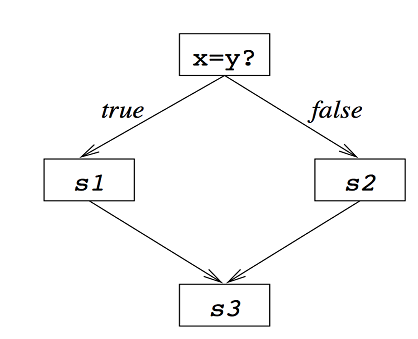
\includegraphics[width=16cm]{img/cfgssa.png}
\caption{Esempio di applicazione dei meccanismi SSA e CFG ad un programma}
\label{fig:cfgssa}
\end{figure}
\subsubsection{Data flow graph}
Il data flow graph mostra il comportamento del modello a livello di operazioni, ed � utile per mostrare il percorso dei dati e per identificare quali operazioni possono essere parallelizzate e quali invece devono per forza essere eseguite in sequenza.\\
Ad ogni blocco base viene associato un DFG nel quale le operazioni sono i nodi e i dati sono i vertici e gli archi esprimono le dipendenze.
Esistono diversi tipi di dipendenze tra i dati:
\begin{itemize}
\item \textbf{Flow} read-after-write
\item \textbf{Anti} write-after-read
\item \textbf{Output} write-after-write
\item \textbf{Input} read-after-read
\end{itemize}
Le dipendenze di tipo \emph{Input} non creano vere dipendenze, mentre le dipendenze di tipo anti e output possono essere rimosse mediante l'utilizzo della tecnica di rinomina dei registri (SSA). A questo punto il DFG individua solamente le dipendenze di tipo \emph{Flow}.
Un esempio di DFG � mostrato riferito al codice di seguto � quello in fig. \ref{fig:dfg}.
\begin{verbatim}
xl = x+dx
ul = u-(3*x*u*))-3*y*dx
yl=y+u*dx
c=xl<a
\end{verbatim}
\begin{figure}[thb]
\centering
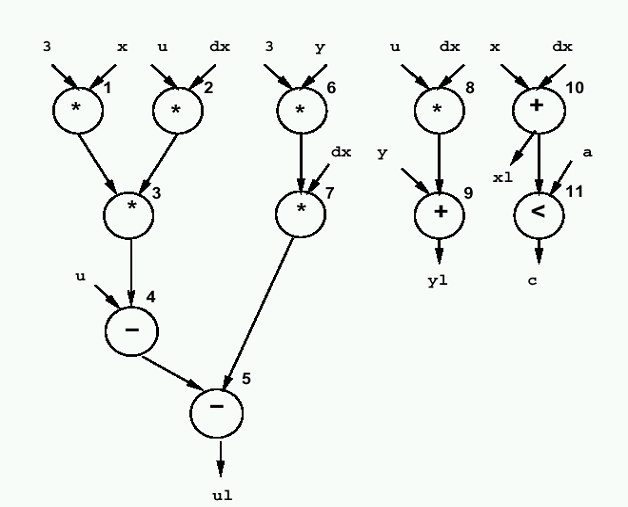
\includegraphics[width=16cm]{img/dfg.png}
\caption{Esempio di Data Flow Graph}
\label{fig:dfg}
\end{figure}
In questo caso noi stiamo ragionando a livello di basic block e quindi le precedenze sono riferite solo al loro interno. Combinando per� il data flow graph e il control flow graph possiamo individuare le precedenze a livello di intero sistema. Un esempio di CDFG � mostrato in fig. \ref{fig:cdfg}
\begin{figure}[t]
\centering
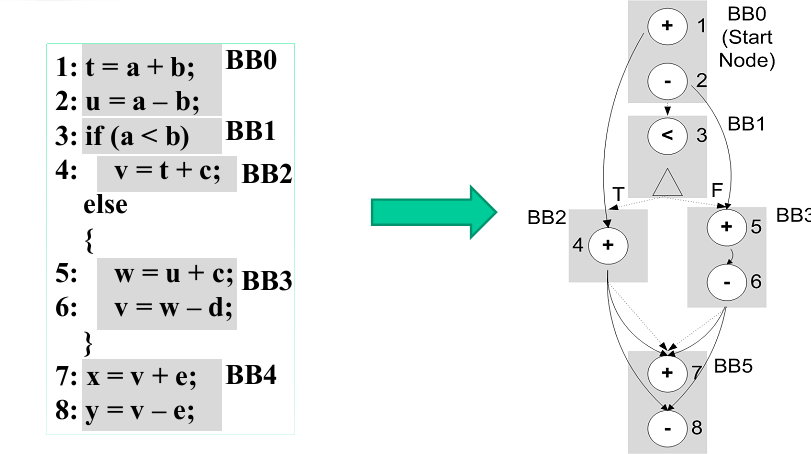
\includegraphics[width=16cm]{img/cdfg.png}
\caption{Esempio di CDFG con relativo codice}
\label{fig:cdfg}
\end{figure}
\subsubsection{Hierarchical Task Graph (HTG)}
A questo bunto risulta complesso per� gestire le ristrutturazioni del sistema; questo non � un problema per grafi di tipo gerarchico \emph{Hierarchical Task Graph} (fig. \ref{fig:htg}).
\begin{figure}[t]
\centering
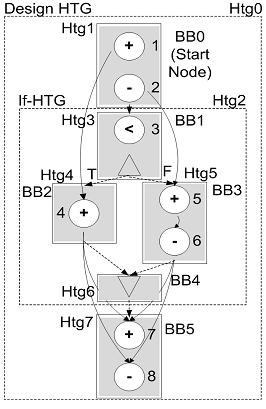
\includegraphics[width=16cm]{img/htg.png}
\caption{Esempio di grafo gerarchico}
\label{fig:htg}
\end{figure}
I grafi di tipo gerarchico mi permettono di individuare quali operazioni potrebbero essere eseguite in parallelo in modo da aumentare le prestazioni del mio sistema.
\subsubsection{Program dependency graph e system dependency graph}
Il \emph{PDG} (Program Dependency Graph) rappresenta il funzinamento di una singola procedura in cui i nodi rappresentano operazioni o predicati di controllo mentre gli archi rappresentano le dipendenze dei dati e di controllo.\\
L'\emph{SDG} (System Dapendency Graph) � una collezione di PDG connessi mediante archi che rappresentano chiamate e passaggi di parametri; esso rappresenta un astrazione del codice nel quale vengono esplicitate le dipendenze e permette un'individuazione pi� facile delle parti di codice parallelizzabili
\subsubsection{Controllo delle dipendenze}
Un nodo A e un dipende da un nodo B se un cambiamento diB fa eseguire o no il nodo A.\\
Una dipendenza di controllo si definisce se Y � controllato dipendentemente da X se e solo se esiste un percorso P da X a Y nel CFG nel quale non esiste un nodo Z in P che � post-domina Y e Y non � post dominato da X.
Tramite questa definizione possiamo distinguere tra le dipendenze fittizie da quelle reali.
\subsection{Tecniche di trasformazione}
Esistono diverse tecniche di trasformazione che servono a modificare il codice in modo da evitare le dipendenze o prepararlo per una fase di ottimizzazione.
Le tecniche principali sono:
\begin{itemize}
\item loop pipelining
\item dynamic renaming
\item copy propagation
\item common subexpression elimination
\item speculative code motion
\item dynamic loop unrolling
\end{itemize}
Partiamo da un codice di esempio e analiziamo alcune tecniche:
\begin{verbatim}
while(k<10)
	sum+=++k;
\end{verbatim}
\begin{figure}[thb]
\centering
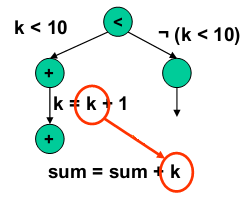
\includegraphics[width=16cm]{img/transform.png}
\caption{DFG del codice di esempio}
\label{fig:transform}
\end{figure}
\paragraph{Loop Pipelining}
Nel caso di loop pipelining si cerca di eseguire le operazioni all'interno del loop in modo pi� possibile parallelo o comunque cercando di anticipare alcune operazioni. Dalla figura \ref{fig:loopP} vediamo come le ultime due operazioni del ramo di sinistra possano essere eseguite in parallelo.
\begin{figure}[hbt]
\centering
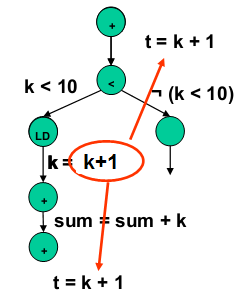
\includegraphics[width=16cm]{img/loopP.png}
\caption{Esempio di loop pipelining}
\label{fig:loopP}
\end{figure}
\paragraph{Copy propagation}
In questo caso si crea una copia di un oggetto che viene propagata in modo da invertire eventuali dipendenze RAW come possiamo vedere in figura \ref{fig:copyP}
\begin{figure}[hbt]
\centering
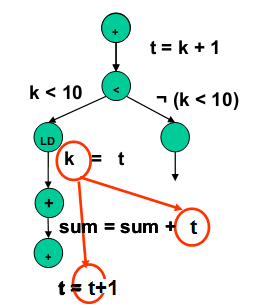
\includegraphics[width=16cm]{img/copyP.png}
\caption{Esempio di copy pipelining}
\label{fig:copyP}
\end{figure}
\paragraph{Speculative Code Motion}
La speculazione � una tecnica che modifica il codice muovendo alcuni blocchi di codice dentro alcuni blocchi base  per lo pi� all'interno di percorsi condizionali. Questo permette di aumentare il parallelismo e massimizzare le risorse utilizzate. Esistono diversi tipi di speculazione:
\begin{itemize}
\item \textbf{Condizionale} nel quale le operazioni eseguite dopo una scelta, ove possibile, vengono portate all'interno delle scelte stesse e la decisione viene presa alla fine dei due rami di scelta.
\item \textbf{Speculation} Le operazioni che si trovano dentro una decisione e che possono essere eseguite in parallelo vengono eseguite prima della decisione stessa e alla fine viene scelto quale risultato utilizzare
\item \textbf{Reverse Speculation} In questo caso i due rami di decisione vengono eseguiti contemporaneamente e le operazioni che si trovavano prima della decisione vengono duplicate all'interno dei due rami.
\item \textbf{Across hierarchical blocks} Operazioni che si trovano dopo due rami di decisione vengono anticipati prima della decisione per aumentarne il parallelismo.
\end{itemize}
Uno schema riassuntivo � mostrato in fig. \ref{fig:speculation}
\begin{figure}[thb]
\centering
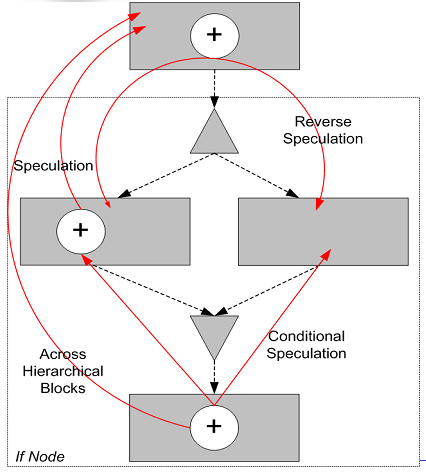
\includegraphics[width=16cm]{img/speculation.png}
\caption{Schema riassuntivo sulla speculazione}
\label{fig:speculation}
\end{figure}
\paragraph{Loop Unrolling}
La tecnica del loop unrolling consiste nel trasformare un normale loop come quello del codice seguente:
\begin{verbatim}
for(i=0; i<32; i++){
	sum=sum+a[i]*b[i];
}
\end{verbatim}
nel seguente ciclo:
\begin{verbatim}
for(i=0; i<31; i++){
	sum=sum+a[i]*b[i];
	sum=sum+a[i+1]*b[i+1];
}
\end{verbatim}
In modo da effettuare una leggera pipelining all'interno del loop e rendere l'albero decisionale pi� "bilanciato" come mostrato in figura \ref{fig:loopunroll}
\begin{figure}[thb]
\centering
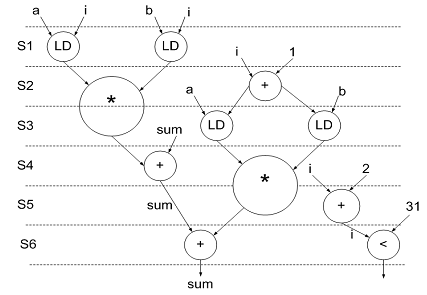
\includegraphics[width=16cm]{img/loopU.png}
\caption{Schema di loop unrolling}
\label{fig:loopunroll}
\end{figure}
\subsection{Lo scheduling}
Per scheduling si intende l'assegnamento dell'ordine di esecuzione alle operazioni nel tempo, possibilmente rispettando vincoli temporali e di hardware sfruttando potenziali parallelismi e cicli.\\
Per risolvere i problemi di scheduling � necessario avere a disposizione il modello del circuito a livello intermedio (soprattutto un CDFG), il tempo di ciclo  e il ritardo delle operazioni, a livello di scheduling � necessario conoscere il tempo di inizio e i vincoli temporali tutto questo tenendo conto del trade-off tra area e ritardo.\\
Il problema di individuare lo scheduling migliore � un problema NP-difficile esistono cos� diverse tecniche euristiche per risolvere tale problema, le pi� comuni sono:
\begin{itemize}
\item ASAP (As soon as possible)
\item ALAP
\item List scheduling, Resource Constrained algorithms
\item Force directed algorithms
\item Path based
\item Percolation algorithms
\item Simulated annealing
\item Tabu search and other heuristics
\item Simulated evolution
\item Linear Programming
\item Integer Linear Programming
\end{itemize}
\paragraph(ASAP)
Partendo dal data flow graph in figura \ref{fig:dfgexe} pensiamo a come "schedulare" le operazioni, ovvero assegnare l'inizio dell'esecuzione delle operazioni a determinati istanti di tempo per. Nel caso in esempio $v_1$, $v_2$, $v_3$, $v_4$, $v_10$ possono partire subito in quanto ricevono degli ingressi primari, essendo i tempi di esecuzione unitari, all'istante \textbf{2} possiamo far partire le operazioni $v_5$, $v_6$, $v_9$ e $v_11$.
Questo scheduling per� tende a sprecare risorse come si pu� vedere nello schema dello scheduling in figura \ref{fig:schedu}.
\begin{figure}[thb]
\centering
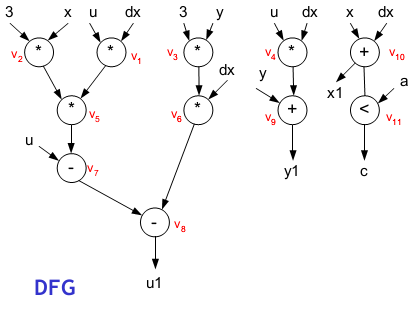
\includegraphics[width=16cm]{img/dfgexe.png}
\caption{Control Data Flow Graph}
\label{fig:dfgexe}
\end{figure}
\begin{figure}[hb]
\centering
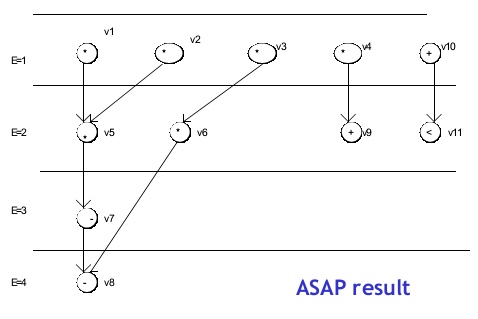
\includegraphics[width=16cm]{img/schedu.png}
\caption{Scheduling ASAP}
\label{fig:schedu}
\end{figure}
Dato uno scheduling posso creare il controllore creando la macchina a stati che implementa quello scheduling per il singolo basic block, componendo tutte le macchine a stati si crea il controllore di tutto il sistema.
\paragraph{ALAP}
Duale rispetto all'algoritmo ASAP l'ALAP risolve i problemi dei vincoli temporali. Il tempo di latenza massimo viene impostato nel tempo di latenza calcolato dall'ASAP e l'ALAP sicuramente rispetter� questo vincolo.\\
Definiamo ora cos'� la mobilit�; essa � riferita ad ogni operazione ed � la differenza tra l'istante di inizio dell'operazione in esame nei due scheduling.
Nel caso una operazione abbia mobilit� uguale a 0 allora significa che lo scheduling di quella operazione in ASAP e in ALAP � uguale. In caso non abbia risorse necessarie per schedulare le operazioni parallelamente, la mobilit� pu� darmi un indice per valutare quali operazioni schedulare per prime per non incrementare la latenza.
\begin{figure}[hb]
\centering
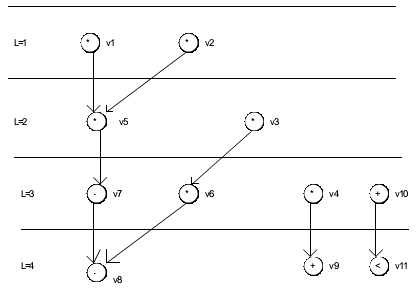
\includegraphics[width=16cm]{img/alap.png}
\caption{Scheduling ALAP}
\label{fig:alap}
\end{figure}
\subsubsection{Scheduling complesso}
Fino ad ora abbiamo visto lo scheduling applicato ad un singolo basic block ora vediamo dato un CDFG completo come costruire lo scheduling completo del sistema.
Come detto prendendo le singole macchine a stati dei singoli basic block e componendole si ottiene la macchina a stati del sistema. Inoltre analizzando le risorse utilizzate dai basic block si ottiene il numero di risorse necessarie per l'esecuzione dell'intero sistema. Si pu� fare ci� perch� i singoli blocchi sono in mutua esclusione.
\subsubsection{Scheduling con vincoli}
In molti casi dobbiamo rispettare alcuni vincoli temporali per quanto riguarda lo scheduling; questi vincoli possono essere sia di tipo massimo ovvero non posso superare un certo limite temporale, ma anche di tipo minimo ovvero non posso completare l'esecuzione prima di un determinato tempo.\\
A questo punto io posso rappresentare questi vincoli nel DFG (fig. \ref{fig:vincoli}) questo permette, tramite opportuni algoritmi, di risolvere il problema dello scheduling.\\
\begin{figure}[t]
\centering
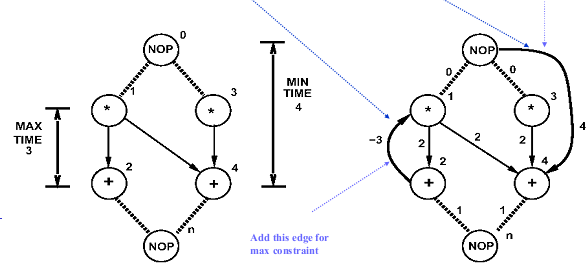
\includegraphics[width=16cm]{img/vincoli.png}
\caption{Esempio di DFG con vincoli temporali}
\label{fig:vincoli}
\end{figure}
\subsection{Resource Binding}
Lo scheduling trascura un componente fondamentale della progettazione, ovvero la distribuzione delle risorse. Il \emph{Resource Binding} pu� essere effettuato in maniera molto banale assegnando alla prima risorsa libera l'operazione da eseguire, ma pi� efficentemente si pu� applicare alcuni meccanismi per l'individuazione dell'allocazione delle risorse e la costruzione del Data Path.\\
Bisogna anche stabilire se il nostro datapath possiede \emph{resource sharing} che non � cos� ovvio nel caso di progetti molto grandi e con costi di interconnessione molto alto.
\subsection{Register allocation}
A questo punto dell'analisi abbiamo costruito il controllore del sistema e le risorse necessarie per eseguire le operazioni. Ora per� dobbiamo rendere disponibile i dati alle risorse; per fare ci� dobbiamo effettuare la \emph{Register Allocation} ovvero stimare quali sono i valori che devono essere memorizzati e individuare quali sono i registri compatibili per memorizzare i dati.
\subsubsection{Scheduled data flow graph}
Lo \emph{Scheduled Data Flow Graph} non � altro che un Data Flow Graph nel quale vengono evidenziati i "confini" delle operazioni come si vede in figura \ref{fig:sdfg}
\begin{figure}[hbt]
\centering
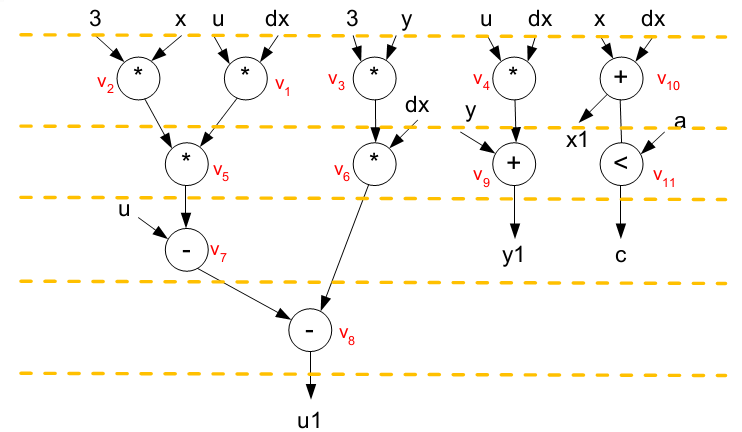
\includegraphics[width=16cm]{img/sdfg.png}
\caption{Scheduled Data Flow Graph}
\label{fig:sdfg}
\end{figure}
In questo schema le linee tratteggiate rappresentano il tempo di inizio e di fine del ciclo di clock e tra un ciclo di clock e l'altro i valori devono essere memorizzati. Perci� per ogni operazione possiamo rifarci allo schema in figura \ref{fig:register} dove possiamo distinguere i registri di lettura e quello di scrittura.
\begin{figure}[thb]
\centering
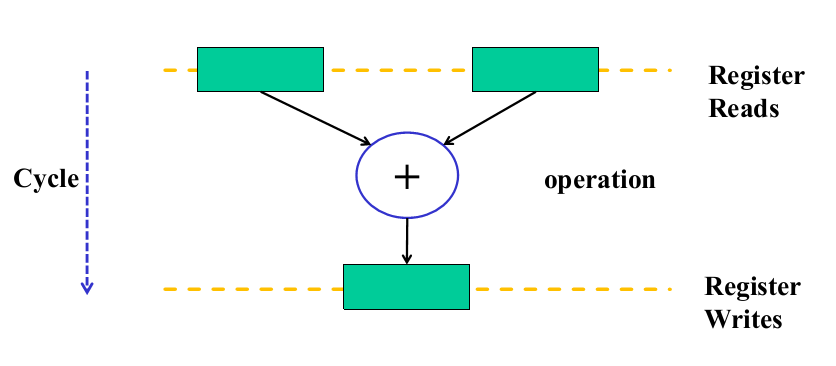
\includegraphics[width=10cm]{img/register.png}
\caption{Schema dei registri}
\label{fig:register}
\end{figure}
Questo � il caso generale per individuare quali variabili debbono essere memorizzate ma esistono altri metodi per individuare i registri, ad esempio:
\begin{description}
\item[Variabili:] in un codice (possibilmente scritto in 3-address form) tutte le variabili rappresentano un registro.
\item[Registri dichiarati:] ovvero i registri vengono dichiarati dai progettisti
\item[Valori:] � quello che abbiamo gi� visto ovvero che ogni arco rappresenta un valore da memorizzare e quindi un registro.
\item[Istanze di valori:] Aggiungere dei valori identici in caso di archi che attraversano pi� cicli di clock. Questo aumenta il grado di libert� sui registri
\item[Istanze limitate di valori:] Simile all'istanze di valori quelle limitate applicano la copia dei valori un limitato numero di volte.
\end{description}
A questo punto abbiamo capito quali sono i possibili registri che dobbiamo allocare come si vede nello schema di figura \ref{fig:register2}
\begin{figure}[hbt]
\centering
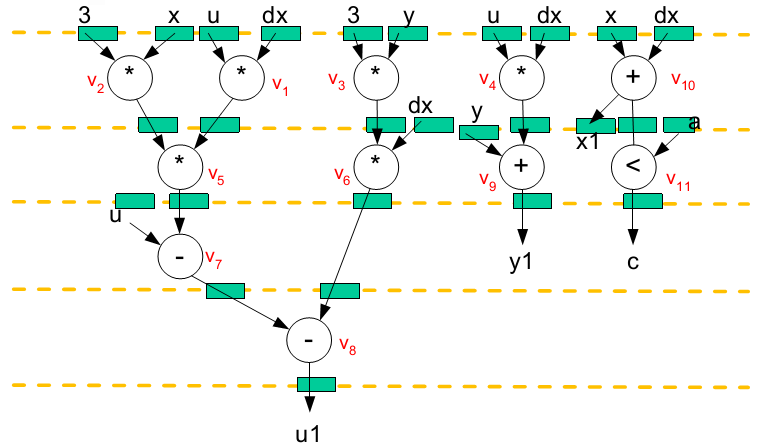
\includegraphics[width=16cm]{img/register2.png}
\caption{SDFG con registri}
\label{fig:register2}
\end{figure}
\subsubsection{Il problema dell'allocazione dei registri}
Il problema che ci poniamo, una volta individuati quali sono i valori da memorizzare, � quello di assegnare ad ogni valore un registro fisico minimizzando il numero dei registri.\\
Nel caso di rappresentazione in SSA automaticamente abbiamo l'insieme degli storage value.\\
Per risolvere il problemanegli anni si � visto che il metodo pi� efficave � l'algoritmo di colorazione dei grafi.\\
Vediamo ora un esempio
\begin{verbatim}
a := c+d;
e := a+b;
f := e-1;
\end{verbatim}
Come si pu� vedere la variabile \emph{a} viene scritta nella prima istruzione e viene letta l'ultima volta nella seconda istruzione, si dice che il suo "tempo di vita" � di una istruzione; per vedere se due storage value sono in conflitto bisogna vedere se i loro tempi di vita si intersecano.
A questo punto riusciamo a costruiro un grafo di interferenza tra gli storage value come quello in figura \ref{fig:storage2} e \ref{fig:storage}
\begin{figure}[thb]
\centering
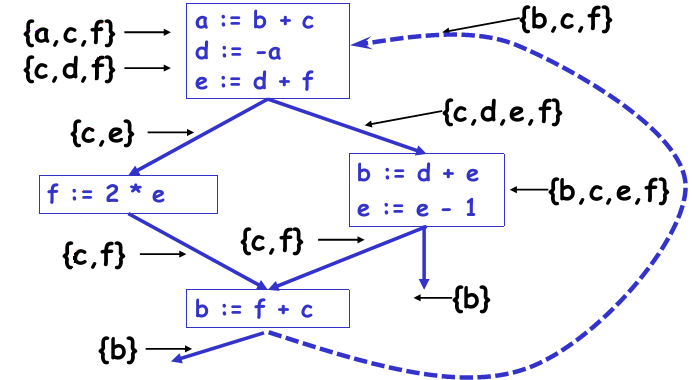
\includegraphics[width=16cm]{img/storage2.png}
\caption{Esempio di grafo di interferenza}
\label{fig:storage2}
\end{figure}
\begin{figure}[thb]
\centering
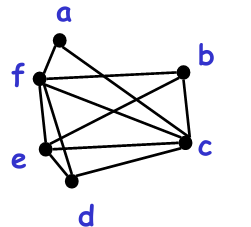
\includegraphics[width=10cm]{img/storage.png}
\caption{Esempio di grafo di interferenza}
\label{fig:storage}
\end{figure}
A questo punto se due storage value hanno archi che li uniscono allora non possono utilizzare lo stesso registro. In questo caso si pu� utilizzare l'algoritmo di un grafo per trovare in maniera ottima il numero di registri minimo.
\subsection{Rilascio delle risorse semplificatrici}
Fino ad ora abbiamo assunto alcune ipotesi per semplificarci le spiegazioni, ora per� vediamo alcune di queste e come eliminarle.\\
La prima ipotesi � che tutte le operazioni avessero lo stesso ciclo di clock. Nella maggior parte dei casi per� questo non � vero, un esempio � dato dal fatto che il moltiplicatore impiega pi� tempo di un sommatore come si vede in figura \ref{fig:udelay},
esistono per� alcune tecniche come il \emph{multicycling} dove un operazione pu� impiegare pi� di un ciclo di clock questo mi permette di dimezzare il ciclo di clock; il \emph{chaing} consiste nel mantenere lo stesso ciclo di clock e di eseguire le operazioni pi� veloce nello stesso ciclo di clock; il \emph{pipelining} consiste di eseguire due operazioni lente in due istanti di clock successivi senza che la prima sia conclusa.
\begin{figure}[t]
\centering
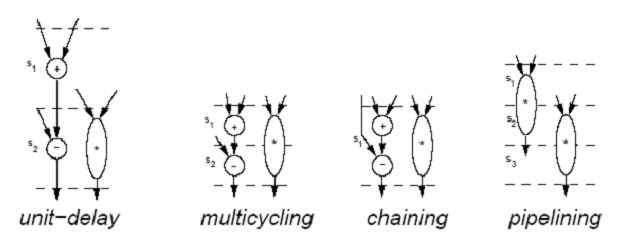
\includegraphics[width=16cm]{img/udelay.png}
\caption{Ottimizzazioni per operazioni multiciclo}
\label{fig:udelay}
\end{figure}


%\label{capitolo6}
\section{Test di circuiti digitali}
I test si collocano dopo la progettazione e dopo la fabbricazione. Questo implica dei problemi di competenza tra pogettisti e fabbricanti. infatti � necessario che tutto ci� che esce dalla progettazione sia oltre che verificato anche testato.\\
Il principio del testing � introdurre un vettore di input in ingresso al circuito e confrontare l'output con la versione corretta.
I test devono coprire il maggior numero di guasti possibili ma non devono essere troppo lunghi.\\
Il modo migliore � analizzare prima i possibili guasti:
\begin{itemize}
\item Individuando i possibili difetti nel processo di produzione
\item Sviluppando simulatori di guasto
\item Sviluppando generatori di test
\item Trovare metodi di quantificazione dell'efficenza dei test.
\end{itemize}Esiste una distinzione tra \emph{verifica} e \emph{test} con il primo termine si intende un meccanismo di analisi che si assicura che il progetto di sintesi assicuri il corretto funzionamento del sistema. Il processo di test, invece, assicura che il sistema fisico non ha difetti.\\
Esistono diversi livelli a cui fare il testing. Il livello pi� basso � quello di chip poi di board ed infine a livello di sistema; il costo di test cresce di un fattore 10 man mano che saliamo di livello nel test.
\subsection{Fault Modeling}
Solitamente i vettore di I/O che si utilizzano nella verifica sono inadeguati per scovare i difetti nella fabricazione in quanto essi sono spesso troppo numerosi e non sempre analizzabili. In questo caso ci viene in soccorso il \emph{fault model} che identifica i punti da testare ed � effettivamente misurabile la quantit� di guasti che si testano.\\
Per progettare un buon modello di test bisogna conoscere i guasti pi� comuni che si possono presentare che sono:
\begin{itemize}
\item apertura o cortocircuito di transitor
\item guasti alla memoria
\item guasti funzionali
\item errori da ritardo
\item errori analogici
\item stuck-at
\end{itemize}
\subsubsection{Guasto stuck-at}
I guasto di tipo stuck-at si ha quando una singola linea \emph{(single stuck-at fault)} mantiene permanentemente il valore 0 o 1 e questo errore comporta un errore in uscita.\\
L'errore di singolo stuck-at � utile per individuare altri tipi di guasti ed inoltre � molto semplice da utilizzare.
Il numero di siti di guasto � dato da:
$n\_ingressi\_primari+n\_porte+n\_bracci\_fanout$
Due guasti $f_1$ e $f_2$ si dicono equivalenti se tutti i test che individuano $f_1$ individuano anche $f_2$. Ogni singolo guasto di un circuito logico pu� essere suddiviso in un sottoinsieme disgiunto nel quale i guasti sono tra loro equivalenti.
\paragraph{Dominanza di guasti}
Se tutti i testi di un qualsiasi guasto $f_1$ individuano un ulteriore guasto $f_2$ allora si dice che $f_2$ domina $f_1$ e si pu� togliere dalla lista dei guasti.
\paragraph{Checkpoints}
Tutti gli ingressi primari e i rami dei fanout vengono chiamati checkpoints. Esiste un teorema che afferma che un test che controlla tutti i guasti su tutti i checkpoints individua tuttti i guasti del circuito.
\subsection{Fault simulation}
Dato un circuito un insieme di vettori di ingresso e un modello di guasto calcolato con i metodi precedenti ci si pone il problema di determinare quale sar� la copertura di guasti testati dall'insieme di vettori di test dati.
Lo scopo principale di questa simulazione � quello di valutare la bont� dei test effettuati e di individuare quelle zone non coperte dai test selezionati.\\
Lo scenario in cui la \emph{fault simulation} si va a collocare � un ambiente in cui abbiamo un circuito logico con diversi livelli di segnale o un sistema ad alto livello nel quale si possono verificare guasti sui singoli pin dei componenti; inoltre i sistemi potranno avere due o tre livelli di segnale per quanto riguarda i circuiti puramente logici o fino a quattro livelli di segnale per i circuiti sequenziali con C-MOS. Infine potremmo avere circuiti ideali con tempi di ritardo nulli per circuiti combinatori e sequenziali o con ritardi negli altri casi.\\
I guasti che andremo ad analizzare saranno di tipo single stuck-at e ove possibile per guasti equivalenti si andr� ad analizzare solo il guasto collassato.\\
\subsubsection{Simulazione seriale}
L'algoritmo consiste nell'ingnettare un singolo guasto in uno dei punti del circuito e di simulare il circuito con guasto con tutti i vettori di ingresso a disposizione e comparando il risultato con quelli salvati. Se la risposta differisce dal risultato previsto si sospende la simulazione e si comunica l'individuazione del guasto.
I vantaggi di questo algoritmo sono la facile implementazione e la grande variet� di quasti che possono essere simulati.\\
Gli svantaggi per� sono che siamo costretti a modificare la netlist del circuito ad ogni simulazione. Esistono per� degli accorgimenti che rendono il sistema meno costoso. Il primo � la verifica se una rete � \emph{fault} o \emph{fault-free} in questo caso si pu� impostare il valore in uscita dalla sottorete al valore errato o corretto a seconda dei casi. Il secondo metodo detto \emph{Mux} prevede di calcolare il valore finale utilizzando oltre all segnale anche il valore di una variabile ausiliaria.
Questo tipo di simulazione per� resta comunque inefficace in quanto richiede simulazioni ripetute e tempi di CPU proibitivi.
\subsubsection{Simulazione parallela}
Si tratta di una tecnica a codice compilato ottima per circuiti con due stati (0,1) sfrutta il parallelismo delle operazioni logiche nei bit delle parole di memoria. Ogni passo della simulazione � in grado di simulare fino a $w-1$ guasti del circuito dove $w$ � la lunghezza della parola; tuttavia questo meccanismo non � sfruttabile per circuiti non booleani o con tempi critici di ritardo.
\begin{figure}[thb]
\centering
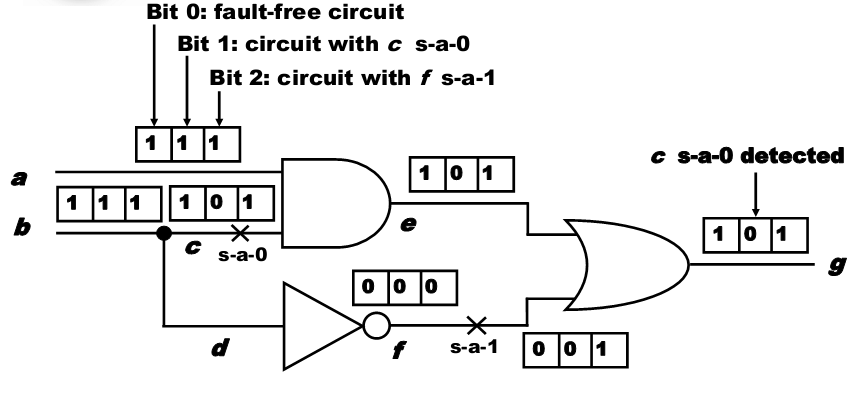
\includegraphics[width=12cm]{img/simul_paral.png}
\caption{Esempio di simulazione parallela}
\end{figure}
\subsubsection{Simulazione di guasto deduttiva}
Questo tipo di simulazione � una simulazione ad un passo; ogni linea k contiene una lista dei possibili guasti che si possono verificare su k. Seguendo i valori della simulazione i valori in uscita dalle porte vengono aggiornati secondo regole teoriche e la lista dei guasti. Il problema della simulazione � che non pu� essere utilizzata su circuiti non booleani a causa delle regole teoriche e i ritardi non vengono ben espressi.
\subsubsection{Simulazione di guasto concorrente}
Una simulazione basata su eventi nel quale si simula il circuito privo di errori e solo quelle parti in cui il guasto causa una differenza di segnale.
Ogni gate contiene una lista di tutte le possibili configurazioni di guasto di quel gate. Ogni possibile configurazione viene simulata. Questo fa si che la simulazione sia molto veloce ma consumi una grande quantit� di memoria.


\end{document}
